% !Tex root = Vorlage.tex
\newpage
\section{Experiments}
A number of experiments has been conducted in order to evaluate the capabilities of empirical risk minimization (ERM) techniques for functional dependency discovery.
For the experiments, datasets from the UCI Machine Learning Repository were used.\cite{DUA19}.
All rows containing missing values are dropped due to possible inconsistencies in the algorithms when handling them.

The measure chosen to compare imputation performance on columns containing continuous numeric values is the mean squared error.
To compare classification performance, the F1-measure is chosen.

\subsection{FD Imputer}
FD Imputer is run for every FD found on a train subset of the Adult dataset.\cite{DUA19}
Figure~\ref{fig:f1_fd_adult} shows the performance of FD Imputer on columns containing classifiable data.
The two top performing FDs have a perfect F1 score of 1 each.
An explanation for this can be found when analyzing the content of columns 4 and 5.

\begin{figure}[ht]
     \centering
     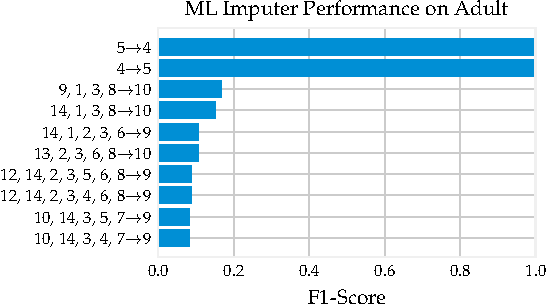
\includegraphics[width=.8\textwidth]{../figures/adult/f1_fd_imputer_adult.pdf}
     \caption{F1 score of the 10 most performant FDs when imputing values on a validation set.}
     \label{fig:f1_fd_adult}
 \end{figure}

Column 4 contains information about the highest educational level achieved.
There are 16 different categories of educational level defined.
Each category is assigned an integer in a range from 0 to 15.
This integer is the content of column 5.
Thus, the relation between column 4 and column 5 can be modeled by a bijective function, projecting the domains of each attribute onto another.

Other FDs lead to F1 scores smaller than \( 0.2\), yielding substantially worse results than the two top-performing FDs.
It can be derived that only the two top-performing FDs hold in a general case.
If unseen data is added to the dataset, it can thus safely be assumed that these two FDs still hold.

\begin{table}[ht]
    \centering
    \begin{tabular}{lrrrrrr}
        \toprule
        & & & \multicolumn{4}{c}{Classification Performance} \\
        \cmidrule(lr{.25em}){4-7}
        Dataset & \# FDs & \# FDs\textsubscript{train} & F1\textsubscript{mean} & F1\textsubscript{max} & F1\textsubscript{min} & \# (F1 = 0) \\
        \midrule
        Adult & 93 & 88 & 0.0669 & 1.0000 & 0.0000 & 10 \\
        Nursery & 11 & 11 & 0.0000 & 0.0000 & 0.0000 & 10 \\
        Iris & & & 0.1274 & 0.2552 & 0.0000 & 1 \\
        Letter & & & & & & \\
        \bottomrule
    \end{tabular}
    \caption{Performance of the FD Imputer on two UCI datasets.}\label{tab:fd-imputer-performance}
\end{table}

Table~\ref{tab:fd-imputer-performance} provides a summary of how FD Imputer performs on the Adult and Nursery datasets.
The column ``\#~FDs'' indicates how many FDs were found on the complete dataset.
``\# FDS\textsubscript{train}'' contains the number of FDs that were detected on the train subset used for imputations.
``F1\textsubscript{mean}'', ``F1\textsubscript{max}'' and ``F1\textsubscript{min}'' indicate the arithmetic mean, maximal and minimal F1 score achieved on each dataset respectively.
The last column named ``\# (F1 = 0)'' provides the number of FDs that scored a F1 score of 0.

The results displayed in table~\ref{tab:fd-imputer-performance} show how strongly the FD Imputer's performance depends on the dataset considered.
On a dataset as normalized as nursery, FD Imputer cannot leverage FDs to impute unknown entries.

\subsection{Datawig Imputer}
Datawig Imputer is run with the same set of FDs as FD Imputer.
The 10 best performing FDs' F1 scores are displayed in figure~\ref{fig:f1_ml_adult}.
\begin{figure}[ht]
     \centering
     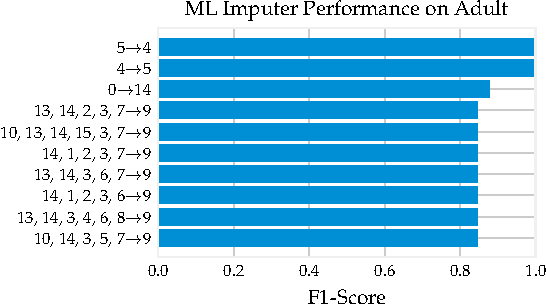
\includegraphics[width=.8\textwidth]{../figures/adult/f1_ml_imputer_adult.pdf}
     \caption{The figure compares the f1-score of the FD Imputer compared to the f1-score of the Datawig Imputer. Each point represents one FD.}
     \label{fig:f1_ml_adult}
 \end{figure}
The two top scoring FDs are the same for FD Imputer and Datawig Imputer.
The third most performant FD is a relation between row ID and nationality.
Since there is no appearent dependency between row ID and nationality, it is safe to assume that Datawig Imputer always guesses the most frequent nationality, US-American, for no matter what row ID.

This shows that Datawig Imputer is capable of learning Conditional Dependencies.

\begin{table}[ht]
    \centering
    \begin{tabular}{lrrrrrr}
        \toprule
        & & & \multicolumn{4}{c}{Classification Performance} \\
        \cmidrule(lr{.25em}){4-7}
        Dataset & \# FDs & \# FDs\textsubscript{train} & F1\textsubscript{mean} & F1\textsubscript{max} & F1\textsubscript{min} & \# (F1 = 0) \\
        \midrule
        adult & 93 & 88 & 0.7720 & 1.0000 & 0.0409 & 0 \\
        nursery & 11 & 11 & 0.4531 & 0.9915 & 0.1138 & 0 \\
        \bottomrule
    \end{tabular}
    \caption{Performance of the Datawig Imputer.}\label{tab:ml-imputer-performance}
\end{table}

Table~\ref{tab:ml-imputer-performance} shows a generally higher performance of Datawig Imputer compared to FD Imputer.
There are no FDs for which Datawig Imputer scores 0.
This can be explained by to Datawig Imputer's behavior of always returning some imputation value, even if certainty is very low.
This is contrasted by FD Imputer, which frequently returns no imputation value at all.

\subsection{Overfitting the Datawig Imputer}

\subsection{Comparing Datawig Imputer with FD Imputer}
As discussed in the previous section, Datawig Imputer and FD imputer differ fundamentally in the way they function.
When comparing the two, metrics need to be computed bearing those differences in mind.

FD Imputer cannot approximate numerical values.
Due to the nature of the definition of a FD, Data is always assumed to be classifiable.
Meanwhile, Datawig Imputer is able to perform regression, predicting a continuous label for a given input with an uncertainty.

Naturally, this circumstance leads to a far superior performance of Datawig Imputer when imputing continuous labels.
FD Imputer usually does not find any values on the train set to impute with and cannot return a meaningful result.
Taking the above into account, rows that aren't imputed by FD Imputer are not considered when computing a performance measure on columns containing continuous values.

\begin{figure}[ht]
     \centering
     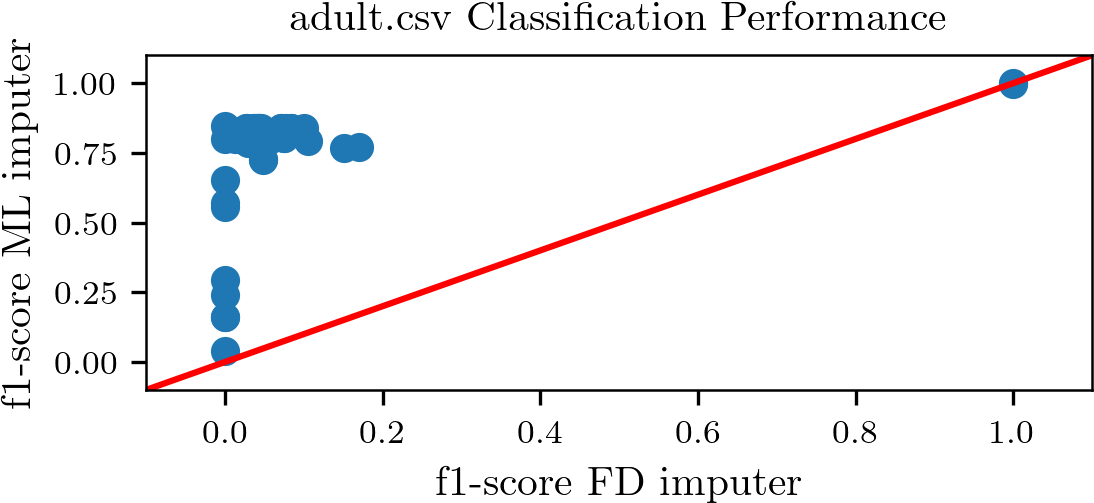
\includegraphics[width=.8\textwidth]{../figures/adult/f1_ml_fd_adult}
     \caption{The figure compares the f1-score of the FD Imputer compared to the f1-score of the Datawig Imputer. Each point represents one FD.}
     \label{fig:f1_ml_fd_adult}
 \end{figure}

Figure~\ref{fig:f1_ml_fd_adult} compares the F1-scores of both Datawig Imputer and FD Imputer on the Adult dataset.
One can observe that for almost all FDs, the Datawig Imputer performs better than the FD Imputer.

FD Imputer performance and Datawig Imputer performance seem to be proportional.
If the ML imputers F1-score is lower than 0.7, the FD Imputers F1-score for the same FD is 0.
However, for FDs where the Datawig Imputer scores are larger than 0.7, the FD Imputer scores better than 0.0.

There are two FDs for which the FD Imputer performs equally good as the Datawig Imputer.
These FDs were identified in the previous section.

\begin{figure}[ht]
     \centering
     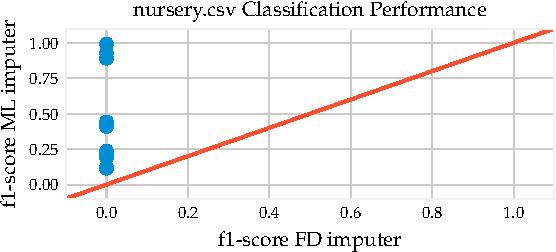
\includegraphics[width=.8\textwidth]{../figures/nursery/f1_ml_fd_nursery}
     \caption{The FD imputers classification performance compared to the performance of the Datawig Imputer on the nursery dataset.}
     \label{fig:f1_ml_fd_nursery}
\end{figure}

The same experiment was run on the Nursery dataset.\cite{DUA19}
Results are displayed in figure~\ref{fig:f1_ml_fd_nursery}.
On this dataset, the ML Imputer performs better for every single FD.
This is explainable by the fact that the Nursery dataset is strongly normalized.
It contains only 11 FDs, most of them are the key, functionally determining a single column.

\subsection{Dependency detection}
Using the approach described in the theory section to detect a generalized imputation dependency, DepDetector is run on number of datasets.
In addition, the stability of discovered minimal dependencies is investigated.

\subsubsection{Dependency stability}
Stability of the found minimal dependency depends on the number of cycles used for training the classifier.
DepDetector is run with different numbers of maximal training cycles.
Minimal dependencies were searched following the `complete' search strategy.

The number of training cycles \( \tau \) is increased stepwise from \( 3 \text{ to } 15 \).
The number of undetected minimal LHSs is calculated by selecting the result of the run with \( \tau = 15 \) training cycles as a reference.
For every time DepDetector is run to find minimal dependencies, the obtained LHSs are compared to the ones obtained with \( \tau = 15 \).
For each LHS found when \( \tau = 15 \) that is not contained in the result of a run, the number of undetected minimal LHSs is increased by one.

Figure~\ref{fig:dep_detector_lhs_stability_iris} shows that the Iris dataset contains two minimal LHS combinations and thus two Dependencies.
For \( \tau \in [7, 15] \) training cycles, DepDetector discovered all minimal dependencies.
\begin{figure}[ht]
     \centering
     \begin{subfigure}[b]{0.45\textwidth}
         \centering
         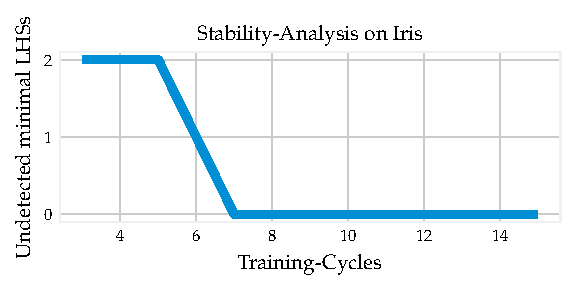
\includegraphics[width=\textwidth]{../figures/iris/iris_dep_detector_lhs_stability}
         \caption{Analysis on the Iris dataset reveals that results become continuously more stable for larger \( \tau \).}
         \label{fig:dep_detector_lhs_stability_iris}
     \end{subfigure}
     \hfill
     \begin{subfigure}[b]{0.45\textwidth}
         \centering
         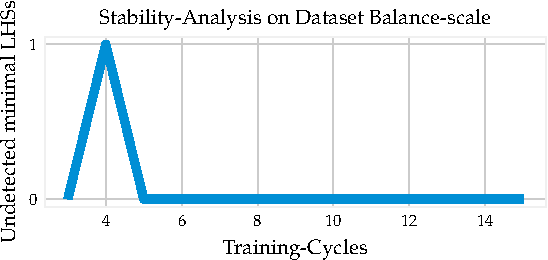
\includegraphics[width=\textwidth]{../figures/balance-scale/balance_scale_dep_detector_lhs_stability.pdf}
         \caption{On the dataset Balance-scale, the analysis of the result shows a peak at \( \tau = 4 \).}
         \label{fig:dep_detector_lhs_stability_balance_scale}
     \end{subfigure}
        \caption{Stability analysis of the minimal LHSs found by DepDetector.}
        \label{fig:stabilit_analysis}
\end{figure}

An analysis on the dataset Balance-scale shows the potentially non-linear behavior of obtained results in function of \( \tau \):
Even though the result obtained for \( \tau = 3 \) is minimal, the result found when \( \tau = 4 \) is in fact not minimal.

For further analysis, DepDetector models are trained with \( \tau = 10 \) training cycles, aiming to detect dependencies that are stable.

\subsubsection{Results on various Datasets}
Dependencies were detected on a number of well-known datasets.
\begin{table}[ht]
    \centering
    \begin{tabular}{lrrrrrrr}
        \toprule
        & & & & & \multicolumn{1}{c}{Greedy} & \multicolumn{1}{c}{Complete} \\
        Dataset & Cols & Rows & \# FDs & \# FDs\textsubscript{train} & \# F1\textsubscript{LHS} $> 0.90$ & \# F1\textsubscript{LHS} $> 0.90$ \\
        \midrule
        adult & 16 & 32561 & 93 & 88 & 99 (100s)& 99 \\
        nursery & 11 & 11 & 99 & 99 & 99 & 99 \\
        abalone & 10 & 4177 & 99 & 99 & 99 & 99 \\
        balance-scale & 6 & 625 & 99 & 99 & 99 & 99 \\
        chess & 8 & 28056 & 99 & 99 & 99 & 99 \\
        iris & 6 & 150 & 99 & 99 & 99 & 99 \\
        letter & 18 & 20000 & 99 & 99 & 99 & 99 \\
        \bottomrule
    \end{tabular}
    \caption{Result of running dependency detection on selected datasets. Values in brackets are the respective algorithm's runtime in seconds.}\label{tab:dep-detection-performance}
\end{table}
